\documentclass[a4paper,10pt]{article}
%\documentclass[a4paper,10pt]{scrartcl}
\usepackage{graphicx}


\usepackage[utf8]{inputenc}

\title{Estimating reconstruction resolution: Fourier Shell Correlation}
\author{Roberto Marabini}
\date{}

\pdfinfo{%
  /Title    ()
  /Author   ()
  /Creator  ()
  /Producer ()
  /Subject  ()
  /Keywords ()
}

\begin{document}
\maketitle

\section{Theoretical Background}

The Fourier Shell Correlation (FSC) estimates the quality (resolution) of a 3D reconstruction. More presisely the FSC  measures the normalised cross-correlation coefficient between two volumes over corresponding shells in Fourier space[1]

\section {Calculation}

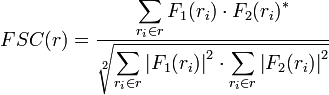
\includegraphics{fsc.png}

\noindent where $F_1$ is Fourier transform for  volume 1, $F_2^{\ast}$ is the complex conjugate of the Fourier transform for volume 2, and $r_i$ is the individual voxel element at radius r. In this form, the FSC takes two three-dimensional data sets and converts them into a one-dimensional array.

\section {Objetive}
Using Matlab implemented the FSC

\section {Bibliography}
[1] Harauz G, van Heel M. Exact filters for general geometry 3--dimensional reconstruction. Optik. 1986;73

\end{document}
